\documentclass[12pt]{book}

\usepackage{natbib} % Tidies up citation numbers.
\usepackage[utf8]{inputenc}
\usepackage{graphicx}
\usepackage{pythonhighlight}
\usepackage{listingsutf8}
\usepackage{float}

%\def\UrlBreaks{\do\/\do-}
\usepackage[T1]{fontenc}
\usepackage{url}
\usepackage{breakurl}

\usepackage{pdfpages}

\lstset{
  extendedchars=true,
  language=java,
  basicstyle=\tiny\ttfamily,
  showspaces=false,
  showstringspaces=false,
    literate=
     {É}{{\'E}}{1}%
      {Á}{{\'A}}{1}%
      {Ã}{{\~A}}{1}%
      {Â}{{\^A}}{1}%
      {À}{{\`A}}{1}%
      {Ç}{{\,C}}{1}%
      {Ó}{{\'O}}{1}%
      {Í}{{\'I}}{1}%
      {Õ}{{\~O}}{1}%
      {Ú}{{\'U}}{1}%
      {ú}{{\'u}}{1}%
      {é}{{\'e}}{1}%
      {á}{{\'a}}{1}%
      {ã}{{\~a}}{1}%
      {à}{{\`a}}{1}%
      {â}{{\^a}}{1}%
      {ç}{{\,c}}{1}%
      {ó}{{\'o}}{1}%
      {í}{{\'i}}{1}%
      {õ}{{\~o}}{1}%
}

\definecolor{gray}{rgb}{0.4,0.4,0.4}
\definecolor{darkblue}{rgb}{0.0,0.0,0.6}
\definecolor{cyan}{rgb}{0.0,0.6,0.6}

\lstdefinelanguage{XML}
{
 numbers=left,
 numberstyle=\tiny,
 stepnumber=1,
 numbersep=8pt,
 morestring=[b]",
 morestring=[s]{>}{<},
 morecomment=[s]{<?}{?>},
 stringstyle=\color{black},
 identifierstyle=\color{darkblue},
 keywordstyle=\color{cyan},
 morekeywords={xmlns,version,type}% list your attributes here
}

\colorlet{punct}{red!60!black}
\definecolor{background}{HTML}{EEEEEE}
\definecolor{delim}{RGB}{20,105,176}
\colorlet{numb}{magenta!60!black}

\lstdefinelanguage{json}{
    basicstyle=\tiny\ttfamily,
    numbers=left,
    numberstyle=\tiny,
    stepnumber=1,
    numbersep=8pt,
    showstringspaces=false,
    breaklines=true,
    frame=lines,
    backgroundcolor=\color{background},
    literate=
     *{É}{{\'E}}{1}%
      {Á}{{\'A}}{1}%
      {Ã}{{\~A}}{1}%
      {Â}{{\^A}}{1}%
      {À}{{\`A}}{1}%
      {Ç}{{\,C}}{1}%
      {Ó}{{\'O}}{1}%
      {Í}{{\'I}}{1}%
      {Õ}{{\~O}}{1}%
      {Ú}{{\'U}}{1}%
      {ú}{{\'u}}{1}%
      {é}{{\'e}}{1}%
      {á}{{\'a}}{1}%
      {ã}{{\~a}}{1}%
      {à}{{\`a}}{1}%
      {â}{{\^a}}{1}%
      {ç}{{\,c}}{1}%
      {ó}{{\'o}}{1}%
      {í}{{\'i}}{1}%
      {õ}{{\~o}}{1}%
     {0}{{{\color{numb}0}}}{1}
      {1}{{{\color{numb}1}}}{1}
      {2}{{{\color{numb}2}}}{1}
      {3}{{{\color{numb}3}}}{1}
      {4}{{{\color{numb}4}}}{1}
      {5}{{{\color{numb}5}}}{1}
      {6}{{{\color{numb}6}}}{1}
      {7}{{{\color{numb}7}}}{1}
      {8}{{{\color{numb}8}}}{1}
      {9}{{{\color{numb}9}}}{1}
      {:}{{{\color{punct}{:}}}}{1}
      {,}{{{\color{punct}{,}}}}{1}
      {\{}{{{\color{delim}{\{}}}}{1}
      {\}}{{{\color{delim}{\}}}}}{1}
      {[}{{{\color{delim}{[}}}}{1}
      {]}{{{\color{delim}{]}}}}{1},
}

\lstdefinelanguage{SPARQL}{
    basicstyle=\tiny\ttfamily,
    numbers=left,
    numberstyle=\tiny,
    stepnumber=1,
    numbersep=8pt,
    showstringspaces=false,
    breaklines=true,
    frame=lines,
    backgroundcolor=\color{background},
    literate=
     {É}{{\'E}}{1}%
      {Á}{{\'A}}{1}%
      {Ã}{{\~A}}{1}%
      {Â}{{\^A}}{1}%
      {À}{{\`A}}{1}%
      {Ç}{{\,C}}{1}%
      {Ó}{{\'O}}{1}%
      {Í}{{\'I}}{1}%
      {Õ}{{\~O}}{1}%
      {Ú}{{\'U}}{1}%
      {ú}{{\'u}}{1}%
      {é}{{\'e}}{1}%
      {á}{{\'a}}{1}%
      {ã}{{\~a}}{1}%
      {à}{{\`a}}{1}%
      {â}{{\^a}}{1}%
      {ç}{{\,c}}{1}%
      {ó}{{\'o}}{1}%
      {í}{{\'i}}{1}%
      {õ}{{\~o}}{1},%
  morekeywords={
    SELECT,CONSTRUCT,DESCRIBE,ASK,WHERE,FROM,NAMED,PREFIX,BASE,OPTIONAL,
    FILTER,GRAPH,LIMIT,OFFSET,SERVICE,UNION,EXISTS,NOT,BINDINGS,MINUS,a
  }
}

\lstdefinelanguage{overpassQL}{
    basicstyle=\tiny\ttfamily,
    numbers=left,
    numberstyle=\tiny,
    stepnumber=1,
    numbersep=8pt,
    showstringspaces=false,
    breaklines=true,
    frame=lines,
    backgroundcolor=\color{background}
}

\lstset{language=R,
    literate=
    {<-}{{$\gets$}}1%
     {É}{{\'E}}{1}%
      {Á}{{\'A}}{1}%
      {Ã}{{\~A}}{1}%
      {Â}{{\^A}}{1}%
      {À}{{\`A}}{1}%
      {Ç}{{\,C}}{1}%
      {Ó}{{\'O}}{1}%
      {Í}{{\'I}}{1}%
      {Õ}{{\~O}}{1}%
      {Ú}{{\'U}}{1}%
      {ú}{{\'u}}{1}%
      {é}{{\'e}}{1}%
      {á}{{\'a}}{1}%
      {ã}{{\~a}}{1}%
      {à}{{\`a}}{1}%
      {â}{{\^a}}{1}%
      {ç}{{\,c}}{1}%
      {ó}{{\'o}}{1}%
      {í}{{\'i}}{1}%
      {õ}{{\~o}}{1},%
    basicstyle=\tiny\ttfamily,
    stringstyle=\color{red},
    otherkeywords={0,1,2,3,4,5,6,7,8,9},
    morekeywords={TRUE,FALSE},
    deletekeywords={data,frame,length,as,character},
    keywordstyle=\color{blue},
    commentstyle=\color{red},
}

\usepackage[brazil]{babel}  
\usepackage{xcolor}
%xcolor v2.12 (2016/05/11)384  Colors by Name4.1  Base colors (always available)black blue brown cyan darkgray gray green lightgray lime magenta olive orange pink purple red teal violet white yellow

\usepackage[nopostdot]{glossaries}
\setglossarystyle{altlist}
\PassOptionsToPackage{hyphens}{url}
\usepackage [colorlinks = true,
            linkcolor = blue,
            urlcolor  = blue,
            citecolor = blue,
            anchorcolor = blue]{hyperref} 

% gerador de lero-lero
\usepackage{lipsum}

\usepackage{pdfpages}

\newenvironment{itquote}
{\begin{quote}\itshape}
{\end{quote}}

\usepackage[commentmarkup=todo]{changes}

\usepackage{datetime2}

\usepackage{booktabs}

\usepackage{caption}
\input{packages-estudantes}

% define cores personalizadas para o texto de cada autor
\usepackage
%[final]
{changes}
%\usepackage{changes}
%\url{https://ctan.org/pkg/changes}

\definechangesauthor[name={Jorge Henrique Cabral Fernandes}, color=orange]{jhcf} % git-user: jhcf

\definechangesauthor[name={Alexsander Correa de Oliveira}, color=black]{KvotheKS} % git-user: KvotheKS OK

\definechangesauthor[name={Allann Gois Hoffmann}, color=orange]{AllannH} % git-user: AllannH OK

\definechangesauthor[name={André Larrosa Chimpliganond}, color=orange]{andrelarrosacrypt} % git-user: andrelarrosacrypt OK

\definechangesauthor[name={André Cássio Barros de Souza}, color=green]{andreloff} % git-user: andreloff OK

\definechangesauthor[name={Bruno Sanguinetti Regadas de Barros}, color=blue]{Jaxiii} % git-user: Jaxiii OK

\definechangesauthor[name={Enzo Nunes Leal Sampaio}, color=orange]{enzodevs2000} % git-user: enzodevs2000 OK

\definechangesauthor[name={Felipe Gomes Paradas}, color=pink]{fparadas} % git-user: fparadas OK

\definechangesauthor[name={Lucas de Almeida Bandeira Macedo}, color=teal]{ABMHub} % git-user: ABMHub OK

\definechangesauthor[name={Fernanda Macedo de Sousa}, color=magenta]{fernandams} % git-user: fernandams Ok

\definechangesauthor[name={Gabriel dos Santos Martins}, color=green]{gsmartins96} %  git-user: gsmartins96 OK

\definechangesauthor[name={Gabriel Faustino Lima da Rocha}, color=gray]{Faustino27} %  git-user: Faustino27 OK

\definechangesauthor[name={Gabriel Martins de Almeida}, color=purple]{GMalme} %  git-user: GMalme OK

\definechangesauthor[name={Gabriel Rocha Fontenele}, color=pink]{ngsylar} % git-user: ngsylar OK

\definechangesauthor[name={Ítalo Eduardo Dias Frota}, color=pink]{titofrota} % git-user: titofrota OK

\definechangesauthor[name={João Antonio Desidério de Moraes}, color=teal]{joaoadm94} % git-user: joaoadm94 OK

\definechangesauthor[name={Ualiton Ventura da Silva}, color=orange]{uventura} % git-user: uventura OK

\definechangesauthor[name={Pedro de Torres Maschio}, color=orange]{pedro-maschio} % git-user: pedro-maschio OK

\definechangesauthor[name={Tong Zhou}, color=orange]{Tong00020} % git-user: Tong00020 Ok

\definechangesauthor[name={Gustavo Rodrigues dos Santos}, color=pink]{gutorsantos} % git-user: gutorsantos OK

\definechangesauthor[name={Gustavo Tomás de Paula}, color=green]{gustavo-tomas} % git-user: gustavo-tomas OK

\definechangesauthor[name={Gustavo Macedo de Carvalho}, color=purple]{GustavoMacCar} % git-user: GustavoMacCar OK

\definechangesauthor[name={Arthur da Silveira Couto}, color=purple]{CrimsonCrown} % git-user: CrimsonCrown OK?

\definechangesauthor[name={Vitor de Oliveira Araujo Araruna}, color=orange]{vitorararuna} % git-user: vitorararuna OK

\definechangesauthor[name={Rafael dos Santos Silva}, color=red]{rafaelsilva21} % git-user: rafaelsilva21 OK

\definechangesauthor[name={Marcus Vinicius Oliveira de Abrantes}, color=red]{MarcusABR} % git-user: MarcusABR OK

\definechangesauthor[name={Mateus de Paula Rodrigues}, color=cyan]{MoustacheGolem} % git-user: MoustacheGolem OK

\definechangesauthor[name={Leonardo Alves Riether}, color=blue]{LeoRiether} % git-user: LeoRiether OK

\definechangesauthor[name={Tatiana Franco Pereira}, color=cyan]{Tatianafp} % git-user: Tatianafp OK

\definechangesauthor[name={Vinícius Caixeta de Souza}, color=orange]{vinis-caixe} % git-user: vinis-caixe OK

\definechangesauthor[name={Conrado Nunes Barbosa Neto}, color=blue]{Conras21} % git-user: Conras21 OK

\definechangesauthor[name={Stefano Luppi Sposito}, color=pink]{KawaiiStheno} % git-user: KawaiiStheno OK

\definechangesauthor[name={João Pedro Felix de Almeida}, color=teal]{DYosplay} % git-user: DYosplay OK

\definechangesauthor[name={João Víctor Siqueira de Araujo}, color=red]{StrawHat972} % git-user: StrawHat972 OK

\definechangesauthor[name={Raylan da Silva Sales}, color=pink]{Rayxan} % git-user: Rayxan OK

\definechangesauthor[name={Guilherme Oliveira Loiola}, color=blue]{guioliunb} % git-user: guioliunb OK

\definechangesauthor[name={Paulo Alvim Alvarenga}, color=purple]{alvimpaulo} % git-user: alvimpaulo OK

\definechangesauthor[name={Léo Akira Abe Barros}, color=red]{leoakir} % git-user: leoakir OK

\definechangesauthor[name={Enzo Yoshio Niho}, color=purple]{enzoyoshio} % git-user: enzoyoshio OK

\definechangesauthor[name={Daniel Rodrigues Cardoso}, color=blue]{DanielrCardoso} % git-user: DanielrCardoso OK

\definechangesauthor[name={Fernando Ferreira Cordeiro}, color=blue]{FernandoCordeiro} % git-user: FernandoCordeiro OK

\definechangesauthor[name={Jônatas Gomes Barbosa da Silva}, color=cyan]{jonatas1n} % git-user: jonatas1n OK

\definechangesauthor[name={Lucas Gabriel de Oliveira Gurgel Fernandes}, color=black]{lggurgel} % git-user: lggurgel OK

\definechangesauthor[name={Bruno Esteves Dalla Costa Filho}, color=red]{brunoedcf} % git-user: brunoedcf OK

\definechangesauthor[name={Paulo Mauricio Costa Lopes}, color=red]{RequiemDosVivos} % git-user: RequiemDosVivos OK

\definechangesauthor[name ={Caio Bernardon Nascif Kaawi Massucato}, color=blue]{CaioMassucato} % git-user: CaioMassucato OK 

\makenoidxglossaries
\loadglsentries{1-Introducao/tarefas/1.1-Glossario/estudantes/main}
\setcounter{tocdepth}{5}
\setcounter{secnumdepth}{5}
\captionsetup[table]{name=Quadro}
\renewcommand{\lstlistingname}{Listagem de Código}

\newcommand{\dataset}{\textit{dataset}}
\newcommand{\query}{\textit{query}}
\newcommand{\githubusername}{\textless githubusername\textgreater}

\begin{document}

\chapter{Análise Bibliográfica sobre o Uso da Tecnologia Blockchain na Área da Saúde, por Bruno Esteves Dalla Costa Filho}

\section{Planejamento do estudo}
A blockchain é um livro-razão compartilhado e imutável que facilita o processo de registro de transações e o rastreamento de ativos em uma rede empresarial. Um ativo pode ser tangível (uma casa, um carro, dinheiro, terras) ou intangível (propriedade intelectual, patentes, direitos autorais e criação de marcas). Praticamente qualquer item de valor pode ser rastreado e negociado em uma rede de blockchain, o que reduz os riscos e os custos para todos os envolvidos.

Ela proporciona segurança de dados para armazenamento devido a criptografia e aos mineradores que verificam cada bloco, tornando a segurança um de seus principais pilares. E de fato, podemos afirmar que o uso do blockchain na saúde é bastante promissor ao garantir segurança extrema de dados, armazenar as informações médicas do paciente e ampliar o acesso ao histórico do paciente, de ensaios clínicos e resultados de novas pesquisas ainda sigilosos.

O estudo do uso da blockchain na área da saúde pode ser focado em:

\begin{itemize}
    \item Quais as possibilidades de uso dessa tecnologia fora da área de finanças?
    \item Como as características da blockchain se encaixam com as necessidades da área da saúde?
\end{itemize}

\subsection{Software de Pesquisa}

Com o uso do Bibliometrix, uma biblioteca da linguagem R amparada pelo R Studio, podemos separar e analisar informações e estatísticas sobre pesquisas científicas e seus temas.

Juntamente com a separação de dados, o Bibliometrix vem com o Biblioshiny que nos proporciona métodos para análise gráfica do estudo realizado, facilitando o entendimento pelo meio visual.

Com o uso dessas duas ferramentas permite a realização do estudo mencionado anteriormente.

\subsection{Limitações}
O estudo foi feito com poucas horas de trabalho graças as facilitações das ferramentas descritas acima.

\section{Coleta de Dados}
A coleta de dados foi feita a partir da base Web of Science no dia 3 de fevereiro de 2022, acessado pelo Portal de Periódicos da CAPES.

\section{Query de Busca}
A busca foi feita apenas com o intuito de encontrar relações entre a tecnologia Blockchain e a Área da Saúde, com um total encontrado de 1126 registros.

\begin{lstlisting}[basicstyle = \normalsize]
    ((blockchain) and (Health))
    \end{lstlisting}

\section{Análise dos dados}

\subsection{Filtragem de registros}
Antes de prosseguir com a análise, uma filtragem dos registros é feita para que se tenha como resultado somente registros de artigos publicados em revistas científicas. Dessa forma, com os 2097 registros inicias, chega-se, no final, ao número de 1834 registros.

\subsection{Análise descritiva do \textit{dataset}}

As informações sobre o \textit{dataset} a partir do Biblioshiny estão descritas a seguir:

\begin{description}
    \item [\textit{Timespan}] Entre os registros obtidos após a filtragem tem-se artigos publicados no período de 2014 a 2022
    \item [\textit{Sources (Journals, Books, etc)}] Obteve-se 584 fonte diferentes para a origem dos registros
    \item [\textit{Average years from publication}] A média do tempo de publicação dos artigos é de 2.09 anos.
    \item [\textit{Average citations per documents}] Cada artigo do \textit{dataset} foi citado em média 11.84 vezes.
    \item [\textit{Average citations per year per doc}] Após a publicação dos artigos, eles foram citados, em média, 3.319 vezes.
    \item [\textit{References}] O total de artigos obtidos possuem juntos 37816 referências citadas.
    \item [\textit{Keywords Plus (ID)}] foram obtidos 906 palavras-chave do tipo Keywords Plus (ID).
    \item [\textit{Author's Keywords (DE)}] 2514 palavras-chave indicadas pelos autores foram encontradas nos registros  .
    \item [\textit{Authors}] 3875 nomes de autores foram encontrados no \textit{dataset}  
    \item [\textit{Author Appearances}] Os 3875 distintos autores foram encontrados 4744 vezes, como autores de artigos.
    \item [\textit{Authors of single-authored documents}] Dentre os 3875 autores encontrados, 60 deles editaram artigos individualmente.
    \item [\textit{Authors of multi-authored documents}] Dentre os 3875 autores encontrados, 3815 deles editaram artigos com um ou mais co-autores.
    \item [\textit{Single-authored documents}] Dentre os artigos encontrados no \textit{dataset}, 62 foram escritos por um único autor.
    \item [\textit{Documents per Author}] Entre os 3875 autores, cada um publicou em média 0.291 documentos.
    \item [\textit{Authors per Document}] Cada um dos artigos encontrados no \textit{dataset} foi autorado, em média, com 3.44 autores.
    \item [\textit{Co-Authors per Documents}] As 4744 aparições autores se distribuem, em média 4.21 vezes para os documentos.
    \item [\textit{Collaboration Index}] Os 3875 nomes de autores que editaram artigos com um ou mais co-autores, colaboraram em media 3.59 vezes.
\end{description}

\subsection{Evolução da produção científica}

Usando o Bibliometrix pode-se obter um gráfico que mostra a produção científica anual sobre o tema em questão. O gráfico obtido é o seguinte:


\begin{figure}[H]
    \centering
    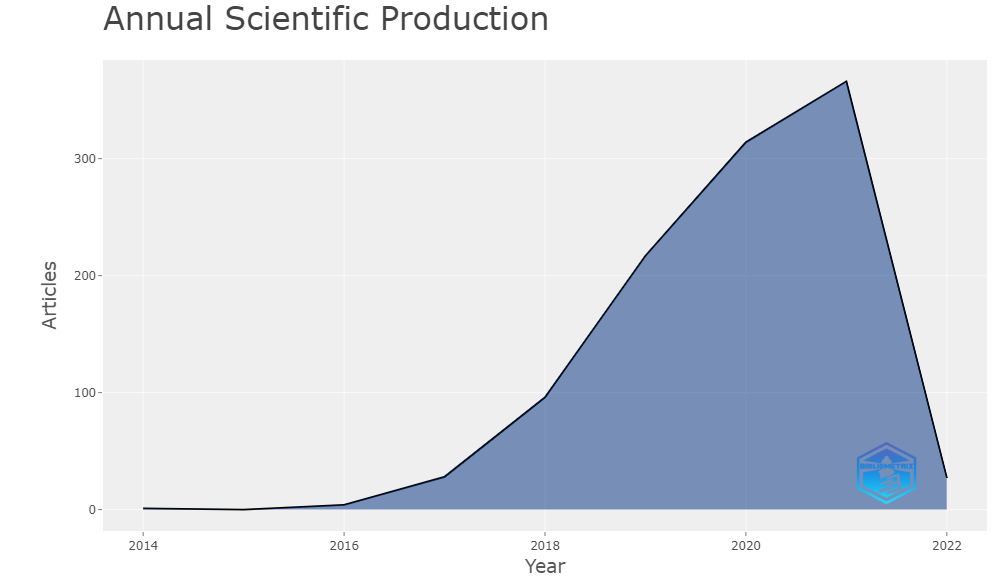
\includegraphics[width=1\textwidth]{experiments/brunoedcf/AnaliseBibliometrica/BlockchainInHealth/Figures/AnualCientProd.png}
    \caption{Evolução da produção científica no \dataset}
    \label{fig:brunoedcf/AnualCientProd}
\end{figure}

Na figura \ref{fig:brunoedcf/AnualCientProd}, o crescimento da produção científica ao longo dos anos relacionando os tópicos Blockchain e Saúde subiu 60.13\%.

\subsection{Interpretação do Crescimento}

O crescimento tem sido mais abrupto ao longo dos anos recentes graças ao impacto no mundo das finanças e criptomoedas em geral. Com bons resultados da tecnologia, surgem discussões sobre seu uso em outras áreas incluindo a da saúde.

\subsection{Evolução das citações}

\begin{figure}[H]
    \centering
    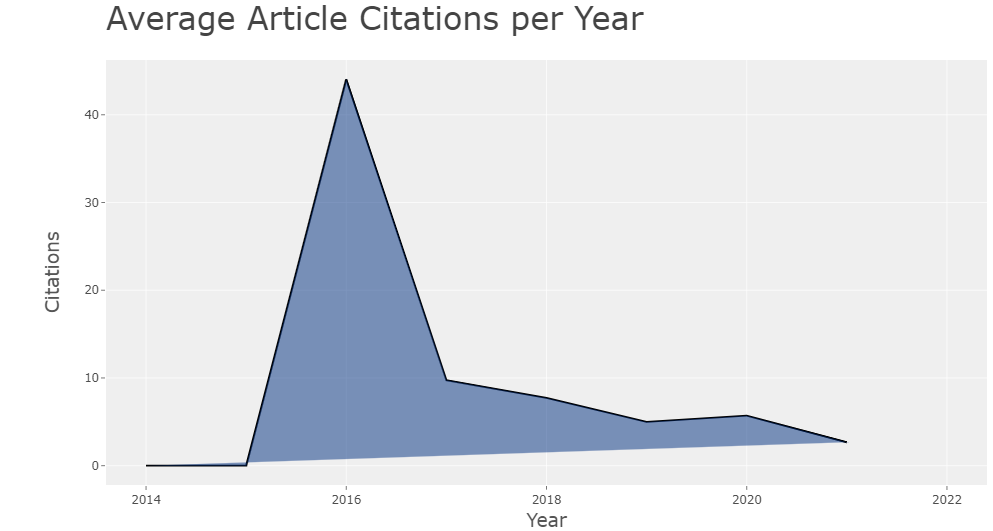
\includegraphics[width=1\textwidth]{experiments/brunoedcf/AnaliseBibliometrica/BlockchainInHealth/Figures/AvgCitationsYear.png}
    \caption{Evolução das citações no \dataset}
    \label{fig:brunoedcf/AvgCitationsYear}
\end{figure}

Na figura \ref{fig:brunoedcf/AvgCitationsYear}, o número médio de citações ao longo dos anos relacionando os tópicos Blockchain e Saúde.

\subsection{Interpretação da Evolução das Citações}

O pico do número de citações por ano se encontrou no ano de 2016 provavelmente devido ao "Boom" das criptomoedas e à introdução da tecnologia em outras partes do mundo das finanças.


\subsection{\textit{Three-Field Plots (Sankey diagram)}}

\begin{figure}[H]
    \centering
    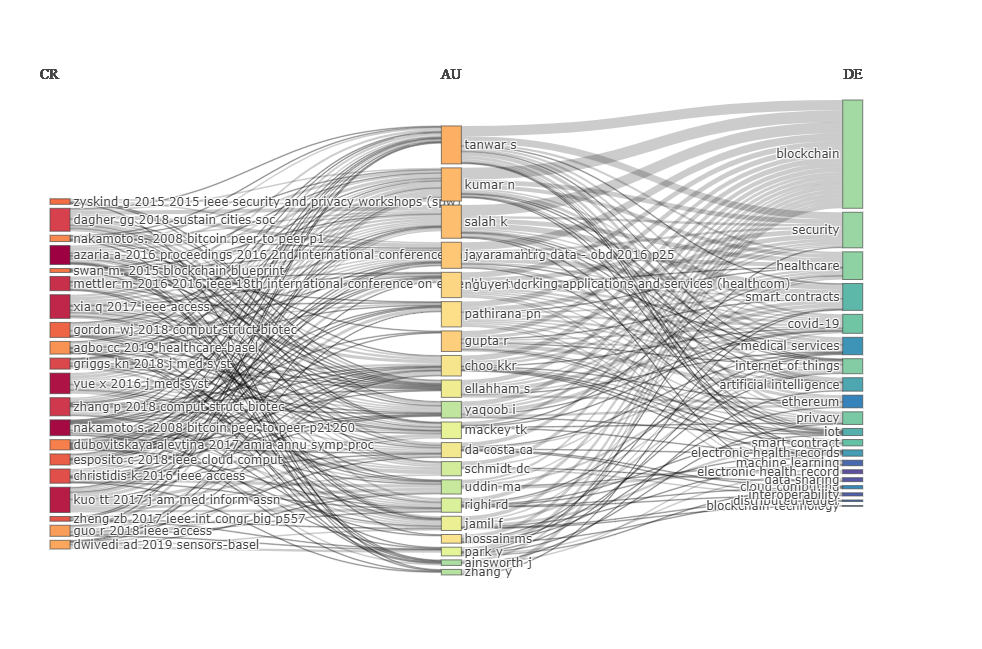
\includegraphics[width=1\textwidth]{experiments/brunoedcf/AnaliseBibliometrica/BlockchainInHealth/Figures/ThreeFieldsPlot.png}
    \caption{Evolução das citações no \dataset}
    \label{fig:brunoedcf/ThreeFieldsPlot}
\end{figure}

O Three-Field Plots (Sankey diagram ou plotagens do tipo “Três Campos”) apresentam afinidades entre três conjuntos de atributos agregados,
vinculando ao centro os 20 Autores mais proeminentes (AU), à esquerda, as 20 Citações mais frequentes (CR - Cited Records), e à direita
as 20 Palavras-Chave mais frequentes empregadas pelos autores.

\subsection{Interpretação da figura \ref{fig:brunoedcf/ThreeFieldsPlot}}

Nas palavras "chave" mais usadas podemos encontrar \textit{security} como a segunda mais utilizada, demonstrando a importância de um dos pilares
da tecnologia blockchain e como pode ser uma das principais razões para sua implementação na área da saúde. 

\section{Refinamento da Coleta de Dados}

Rede de co-ocorrência de palavras aplicada ao \textit{dataset} para filtragem de relações e temas relacionandos entre artigos.

\begin{figure}[H]
    \centering
    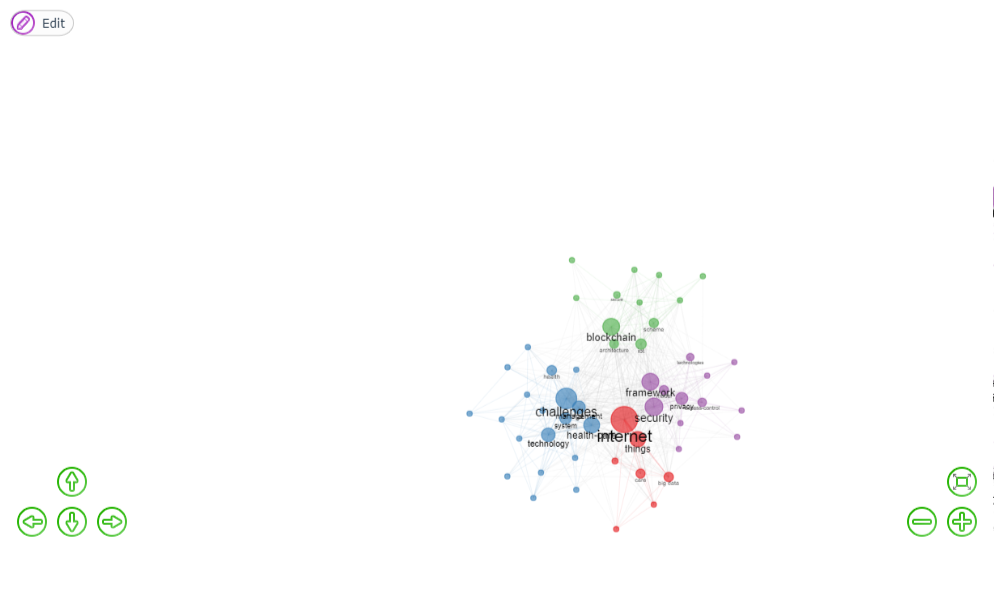
\includegraphics[width=1\textwidth]{experiments/brunoedcf/AnaliseBibliometrica/BlockchainInHealth/Figures/WordOccurrNet.png}
    \caption{Evolução das citações no \dataset}
    \label{fig:brunoedcf/WordOccurrNet}
\end{figure}

O conjunto das palavras consideradas "chave" na busca foram: 

internet, challenges, blockchain, security, health-care, framework.



\bibliographystyle{plainnat}
\bibliography{RESIC}

\end{document}.
